\documentclass{beamer}

% importations de packages utiles
\usepackage[utf8]{inputenc}  % pouvoir écrire avec des accents
\usepackage[french]{babel}  % francophopnie
\usepackage{hyperref}  % liens clicables dans pdf final
\usepackage{tikz}  % pouvoir tracer des dessins sympas
\usetheme{Boadilla}  % thème de beamer
\usepackage{listingsutf8}  % rendu de "code" (avec config ci-dessous)
\definecolor{lstcolor}{rgb}{0.9,0.95,0.95}
\definecolor{lstcommentcolor}{rgb}{0.,0.2,0.}
\lstset{
  frameround=tttt,
  %autogobble,
  frame=single,
  backgroundcolor=\color{lstcolor},
  % extendedchars=true,
  % basicstyle=\ttfamily\small,
  keywordstyle=\bfseries\color{blue},
  identifierstyle=\bfseries\color{red},
  stringstyle=\bfseries\color{orange},
  commentstyle=\color{lstcommentcolor},
  language=Python,
  keepspaces=True,
  basicstyle=\fontfamily{pcr}\selectfont\small, % monospace it for copypasting
  upquote=true,
  columns=flexible,
  showstringspaces=False,
  literate={é}{{\'e}}1
           {â}{{\^a}}1
           {à}{{\`a}}1
           {ç}{{\c c}}1
}
\usepackage[most]{tcolorbox}
\newtcbox{\codebox}{nobeforeafter,tcbox raise base,
  boxrule=0pt,top=0mm,bottom=0mm,
  right=0mm,left=0mm,arc=0pt,boxsep=1.5pt,before upper={\vphantom{dlg}},
  % fontupper=\ttfamily, % <-- seems to have no effect
  colback=gray!50!white,
  }
\robustify{\codebox}
\newcommand\code[1]{\codebox{#1}}
\newcommand\minitoc{
  \begin{frame}{\secname}
    \tableofcontents[currentsection, hideothersubsections, ] %  sectionstyle=show/show]
  \end{frame}
}
\newcommand\ignore[1]{}

\title{La Concurrence}
\subtitle{Concepts de Langages de Programmation}
\author{Juan-Carlos Barros et Daniel Kessler}
\date{juin 2021}
% et c'est parti
\begin{document}
\begin{frame}
  \titlepage
\end{frame} % titre
\begin{frame}{La Concurrence}
  \tableofcontents[hidesubsections]
\end{frame} % toc

\section{Introduction}
\minitoc
\subsection{Définition de la concurrence}
\begin{frame}{Définition}
  \begin{center}
    \begin{minipage}{.7\linewidth}
      La \textbf{concurrence} en informatique consiste en l'exécution de
      plusieurs \textbf{tâches} simultanément (pendant des
      périodes qui se chevauchent) plutôt que séquentiellement (l’une démarrant
      après la fin de l’autre).
    \end{minipage}    
  \end{center}
\end{frame} % définition
\subsection{Le cerveau \textit{vs}\, le \textsc{cpu}}
\begin{frame}{La concurrence est en nous}
  Le \textbf{cerveau} est intrisèquement \textbf{concurrent}.
  \par\bigskip
  \begin{minipage}{.6\textwidth}
    \begin{itemize}
    \item<2-> traitement du stimulus visuel
    \item<3-> traitement du stimulus auditif
    \item<4-> traitement de la syntaxe, grammaire puis sémantique
    \item<5-> analyse du sens
    \item<6-> comparaison avec les connaissances mémorisées
    \item<7-> critique
    \end{itemize}
  \end{minipage}
  \onslide<2->{\;
  \begin{minipage}{.35\linewidth}
    \Large
    Ce mot est {\color{green}{rouge}}.
    \par\bigskip
    Ce mot est {\color{blue}{vert}}.
    \par\bigskip
    Ce mot est {\color{red}{bleu}}.
    \par\bigskip\bigskip
  \end{minipage}}
\end{frame} % cerveau parallèle
\begin{frame}
  \frametitle{La séquence est dans l'ordinateur}
  Le \textbf{processeur} est intrinsèquement \textbf{séquentiel}.\par\bigskip
  \begin{minipage}{.55\textwidth}
    \begin{itemize}
    \item Une instruction exécutée à la fois
    \item<2-> Pourquoi chercher la concurrence?
      \begin{itemize}
      \item<3-> Interruptions I/O
      \item<4-> Exécuter plusieurs programmes ``simultanément''
      \item<5-> Systèmes distribués
      \end{itemize}
    \end{itemize}
  \end{minipage}\quad
  \begin{minipage}{.4\textwidth}
    \begin{center}
      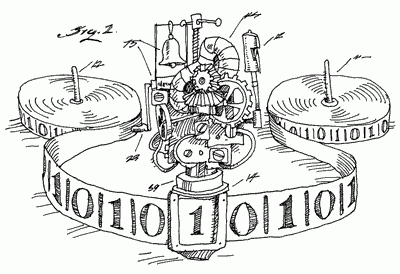
\includegraphics[width=.8\textwidth]{turing.png}
    \end{center}
  \end{minipage}
\end{frame} % cpu séquentiel
\subsection{Le système d'exploitation}
\begin{frame}
  \frametitle{OS: le maître de la concurrence}
  Le \textbf{système d'exploitation} est un ``magicien''.
  \par\bigskip
  \begin{minipage}{.55\textwidth}
    \begin{itemize}
    \item<2-> gestion des ressources séquentielles
    \item<3-> couches d'abstraction
    \item<4-> partage des ressources:\par
      $\rightarrow$ \textbf{l'ordonnanceur}
      \begin{itemize}
      \item<5-> gestion des priorités
      \item<6-> commutation des contextes
      % \item gestion des dangers de la concurrence
      \end{itemize}
    \end{itemize}
  \end{minipage}
  \begin{minipage}{.44\textwidth}
    \begin{center}
      
\includegraphics[width=.7\textwidth]{os.png}
    \end{center}
  \end{minipage}
\end{frame} % l'OS

\section{Mémoire partagée: un problème critique}
\minitoc
\subsection{Les fondamentaux de la concurrence}
\begin{frame}
  \frametitle{Les fondamentaux de la concurrence}
  Comment se manifeste la concurrence? (répartition des tâches)
  \begin{itemize}
  \item multiplicité des \textbf{processus}
  \item multiplicité des \textbf{fils d'exécution} (threads)
  \end{itemize}
\par\bigskip
  Comment communiquent les différents composants?
  \begin{itemize}
  \item via des \textbf{ressources communes}
  \end{itemize}
\end{frame} % la concurrence, comment?
\subsection{Problèmes et solutions}
\begin{frame}
  \frametitle{Problèmes et solutions}
  \begin{minipage}{.49\textwidth}
    Problèmes
    \begin{itemize}
    \item Situation de compétition
    \item Inversion de priorité
    \item Entrelacement
    \item Interblocage
    \item Famine
    \item etc.
    \end{itemize}
  \end{minipage}
  \begin{minipage}{.49\textwidth}
    Solutions
    \begin{itemize}
    \item Verrous
    \item L'Atomicité
    \item Les Moniteurs
    \item Les Sémaphores
    \item Futures et Promises
    \item Et d'autres paradigmes
    \end{itemize}
  \end{minipage}
\end{frame} % problèmes et solutions
\begin{frame}
  \frametitle{Problème 1: \textbf{interleaving} (``entrelacement'')}
  Déterminisme ou indéterminisme?
  \begin{itemize}
  \item programme séquentiel: toujours déterministe
  \item programme concurrent: peut être déterministe
    \par$\rightarrow$
    toutes les possibilités d'entrelacement doivent été prises en compte!
    \par$\rightarrow$
    prouver la validité d'un programme concurrent est particulièrement ardu!
  \item Si le résultat dépend de l'ordre d'exécution, le déterminisme est perdu
  \end{itemize}
\end{frame} % interleaving
\begin{frame} 
  \frametitle{Problème 2: \textbf{race condition}}
  \begin{minipage}{.48\textwidth}
    Deux tâches pourraient tenter d'accéder à une même partie
    de leur mémoire partagée simultanément, ce qui dans la pratique
    pourra poser problème.
  \end{minipage}
  \quad
  \begin{minipage}{.45\textwidth}
    \begin{center}
      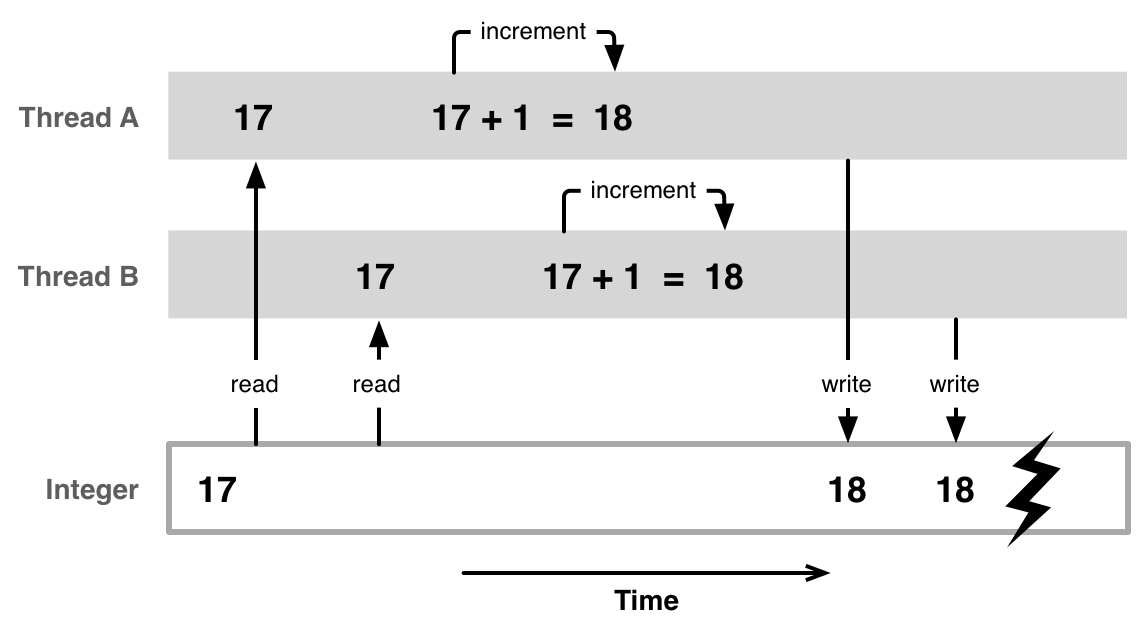
\includegraphics[width=.7\textwidth]{race-condition.png}      
    \end{center}
  \end{minipage}
\end{frame} % race condition
\begin{frame}
  \frametitle{Solution 1: \textbf{verrou} (lock)}
  Un \textbf{verrou} limite l'accès d'une ressource à une seule tâche.
  \begin{itemize}
  \item état fermé vs. état ouvert
  \item si le verrou est fermé, les tâches sont bloquées
  \item sinon, une tâche qui accède à la ressource ferme le verrou
  \item quand la tâche finit, elle ouvre le verrou
  \end{itemize}
\end{frame} % verrou
\begin{frame}
  \frametitle{Solution 2: \textbf{sémaphore} de Dijkstra}
  \begin{minipage}{.7\textwidth}
    \begin{itemize}
    \item Inventé pour l'OS ``THE operating system''
    \item Compteur de tâches en attente de la ressource
    \item 3 primitives
      \begin{itemize}
      \item \texttt{Init(sem, max)} définit nombres d'utilisateurs max
      \item \texttt{P(sem)} pour accéder à la ressource
      \item \texttt{V(sem)} pour quitter la ressource
      \end{itemize}
    \item \texttt{P(sem)} bloque si max atteint, sinon incrémente le compteur
    \item \texttt{V(sem)} décrémente le compteur et notifie les tâches en
      attente
    \item cas particulier: \textbf{sémaphore binaire} ou \textbf{mutex} quand \texttt{max=1}.
    \end{itemize}
  \end{minipage}
  \begin{minipage}{.28\textwidth}
    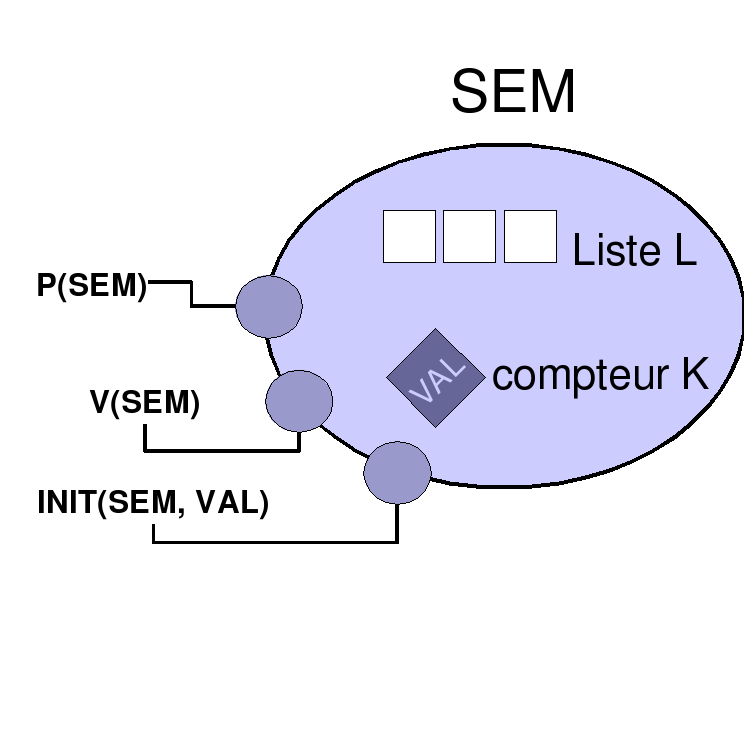
\includegraphics[width=.7\textwidth]{semaphore.png}
  \end{minipage}
\end{frame} % sémaphore
\begin{frame}
  \frametitle{Solution 3: \textbf{moniteur} (Hoare / Brinch-Hansen)}
  \begin{minipage}{.49\textwidth}
    \begin{itemize}
    \item Inventé pour \textit{Equivalent Pascal} et \textit{Solo operating
        system}
    \item Verrou avec une ou plusieurs \textbf{conditions}
    \item Condition liée à \textbf{file d'attente} de processus voulant
      accéder à une ressource
    \item Équivalence avec sémaphores
    \end{itemize}
  \end{minipage}
  \begin{minipage}{.49\textwidth}
    \begin{center}
    \only<1>{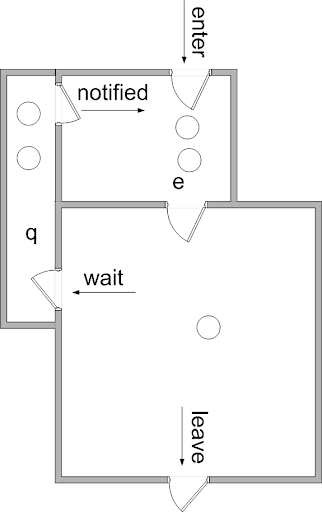
\includegraphics[width=.5\textwidth]{monitor2.png}}
    \only<2>{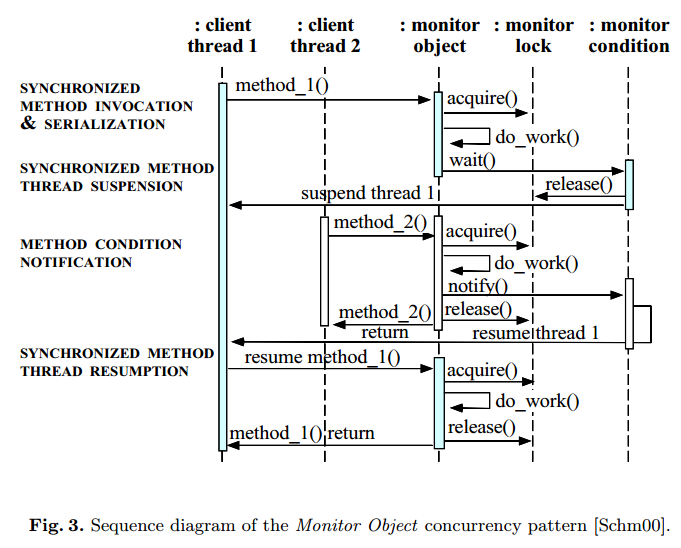
\includegraphics[width=.9\textwidth]{monitor.png}}      
    \end{center}
  \end{minipage}
\end{frame} % moniteur
\begin{frame}[containsverbatim]{Solution 3: \textbf{moniteur} (Hoare / Brinch-Hansen)}
\begin{lstlisting}[language=Java]
public class SynchronizedCounter {
  private int c = 0;

  public synchronized void increment() {
    c++;
  }

  public synchronized void decrement() {
    c--;
  }

  public synchronized int value() {
    return c;
  }
}
\end{lstlisting}}
\end{frame} % moniteur Java
\begin{frame}
  \frametitle{Problème 3: \textbf{interblocage} et \textbf{famine}}
  \begin{minipage}{.55\textwidth}
    Verrous, etc. $\Rightarrow$ nouveaux problèmes!\ldots
    \bigskip
    \begin{itemize}
     \item Deux tâches pourraient chacune verrouiller une ressource dont l'autre
       à besoin\par
       $\rightarrow$ \textbf{interblocage}
     \item Une tâche attend indéfiniment une ressouce bloquée\par
       $\rightarrow$ \textbf{famine}
     %\item Une tâche prioritaire bloquée cède sa place à une tâche de priorité
     %  faible $\rightarrow$ \textbf{inversion de priorité}
    \end{itemize}
  \end{minipage}
  \;\;
  \begin{minipage}{.39\textwidth}
    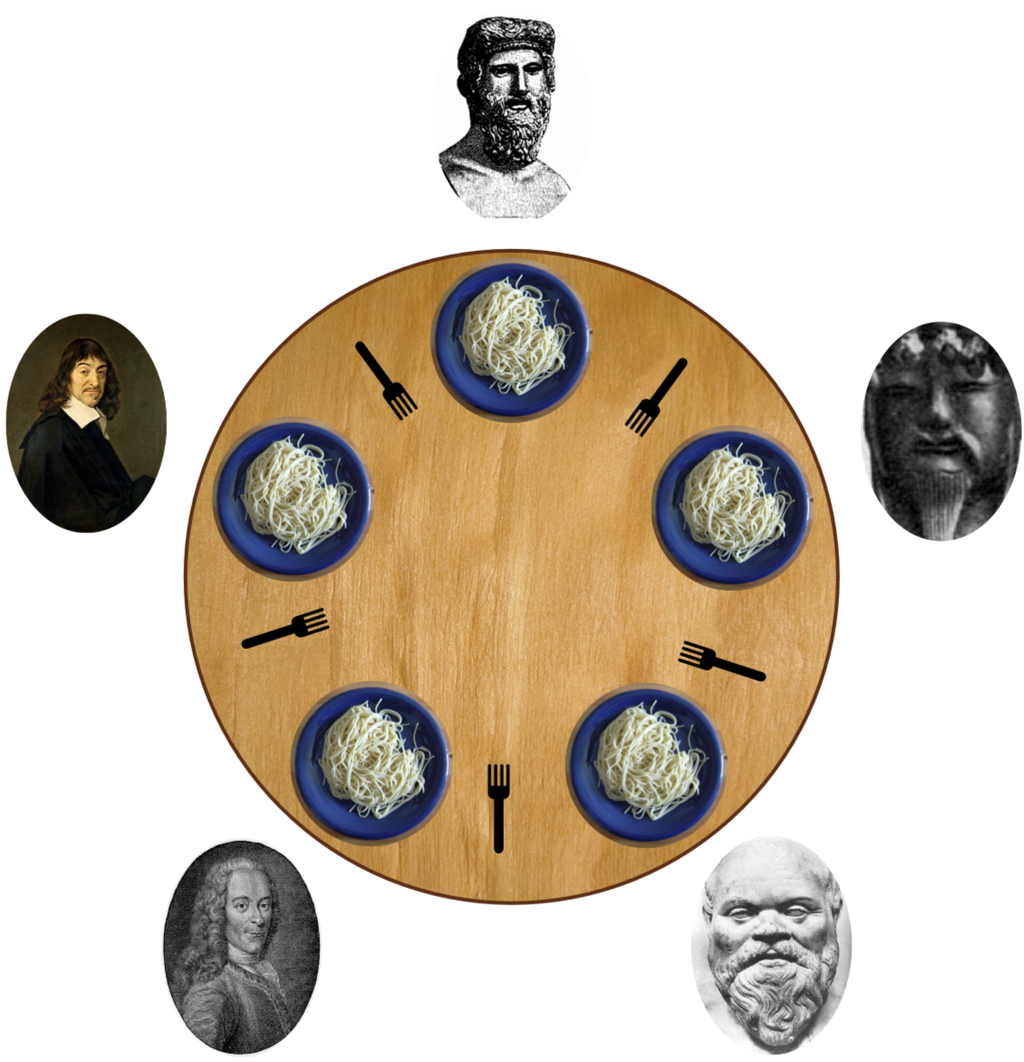
\includegraphics[width=.7\textwidth]{philosophes.png}
  \end{minipage}
\end{frame} % interblocage et famine
\begin{frame}
  \frametitle{Solution 4: Futures et Promises}
  % \begin{minipage}{.5\textwidth}
  Les \textbf{Futures} et \textbf{Promises} sont des abstractions
  de plus haut niveau que les verrous, sémaphores ou moniteurs.
  \bigskip

  Un Future/Promise est une valeur qui peut déjà être disponible, ou sinon,
  devrait devenir disponible plus tard.
  \bigskip

  La distinction entre les deux est floue et dépend du langage de
  programmation.

  Si distinction il y a, le Future apparaît comme un objet
  ``en lecture seule''.
\end{frame} % futures et promises

\section{Côté pratique}
\minitoc
\subsection{Implémenation naïve}
\begin{frame}[containsverbatim]{Implémenation naïve d'un Future minimal en Python}
\begin{lstlisting}
class FutureNaif:
  """Future implémenté "à la main", avec thread privé."""

  def __init__(self, task):
      """Initialiser un Future."""
      self.done = False
      self.result = None
      self._task = task
      # pas besoin de lock vu que le thread est créé
      # sur place et n'est référencé nulle part ailleurs
      self.__thread = threading.Thread(target=self._target)
      self.__thread.start()

  def _target(self):
      """Travail à effectuer par le thread dédié."""
      self.result = self._task()
      self.done = True    
\end{lstlisting}
\end{frame}
\subsection{Thread/Process Pools}
\begin{frame}{Thread/Process Pools et Executors}
  \begin{center}
    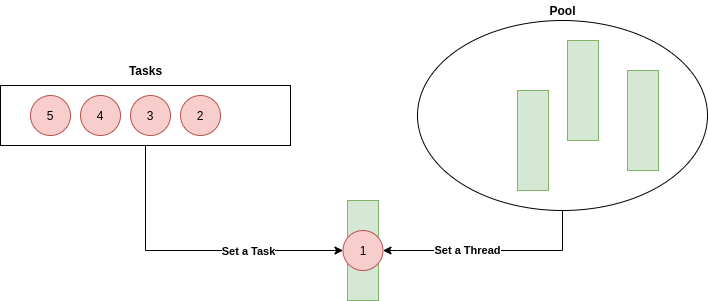
\includegraphics[width=.7\textwidth]{threadpool.png}
  \end{center}
\end{frame}
\subsection{Tests de performance}
\begin{frame}{Tests de performance}
  Comparaison de deux situations\ldots
  \begin{itemize}
  \item Calcul intensif
  \item I/O avec latence
  \end{itemize}
\bigskip
\onslide<2->{\ldots en utilisant trois approches:
  \begin{itemize}
  \item séquentielle
  \item concurrente par \textit{threads} (garantis non parallélisés)
  \item concurrente par \textit{process} (garantis parallélisés)
  \end{itemize}
  }
\end{frame} % Futures en Python

\section{Changement de paradigme}
\minitoc
\subsection{Autres manières d'utiliser des futures}
\begin{frame}[containsverbatim]{Future avec \textbf{callback} associé (exemple en Scala)}
\begin{lstlisting}[language=Scala]
import scala.concurrent.Future
import scala.concurrent.ExecutionContext.Implicits.global
import scala.util.{Failure, Success}

object ScalaFuture extends App {

  val finiraPlusTard = Future {
    ... // tâche longue
  }

  finiraPlusTard.onComplete {
    case Success(valeur) => traiterValeurDeRetour(valeur)
    case Failure(exception) => gererException(exception)
  }

  Thread.sleep(2000)  // "garder en vie" le runtime
}
\end{lstlisting}
\end{frame} % Futures avec callbacks (Scala)
\begin{frame}[containsverbatim]{\textbf{pipelining} de Promise (exemple en javascript)}
  \begin{lstlisting}[language=java]
function faireQuelqueChose() {
   // ...
     return new Promise(...)
   }

faireQuelqueChose()
  .then(x => faireAutreChose(x))
  .then(x => faireUneTroisiemeChose(x))
  .then(x => {
       console.log("Résultat final reçu: ${x}");
    })
  .catch(gererEchec);
\end{lstlisting}
\end{frame} % promises enchaînées (javascript)
\subsection{Les fondamentaux de la concurrence (2)}
\begin{frame}
  \frametitle{Les fondamentaux de la concurrence (2)}
  Comment se manifeste la concurrence? (répartition des tâches)
  \begin{itemize}
  \item multiplicité des \textbf{fils d'exécution} (threads)
  \item multiplicité des \textbf{processus}
  \item<2-> multiplicité des processeurs
  \item<2-> multiplicité des machines
  \end{itemize}

  Comment communiquent les différents composants?
  \begin{itemize}
  \item via des \textbf{ressources communes}
  \item<3-> de manière \textbf{synchrone}: transmission d'information directe
  \item<3-> de manière \textbf{asynchrone}: transmission d'information indirecte
  \end{itemize}
\end{frame} % la concurrence, comment?
\begin{frame}
  \frametitle{Éviter la mémoire partagée?}
  \begin{itemize}
  \item La mémoire partagée était la source de la plupart des problèmes
    \par\bigskip
    $\Rightarrow$ l'éviter ou la cacher dans une couche d'abstraction qui la
    gère de manière automatique et efficace
  \item<2-> Les communications ne devraient se faire que par \textbf{messages} ou \textbf{événements}
  \item<3-> Les messages ou événements ne devraient être constitué que de données \textbf{immuables}
  \end{itemize}
\end{frame}
\subsection{Modèle d'Acteurs de Hewitt}
\begin{frame}{Modèle d'Acteurs de Hewitt}
  Un \textbf{acteur} peut:
  \begin{itemize}
  \item Envoyer des \textbf{messages} à d'autres acteurs
  \item Créer d'autres acteurs
  \item Décider de son comportement à la prochaine réception de message
  \end{itemize}
\end{frame} % déf Acteurs
% \begin{frame}{Futures dans le modèle Acteurs}
% \end{frame} % Futures dans modèle Acteur
\begin{frame}[containsverbatim]
  \frametitle{Modèle d'Acteurs en Erlang}
  Le langage \textbf{Erlang} exploite bien ce modèle.
  \begin{center}
\begin{lstlisting}[language=erlang]
-module(acteur).
-export([start/0, alice/0]).

alice() ->
    receive
        hello ->
            io:format("Alice dit bonjour.~n", [])
    end.

start() ->
    Alice_PID = spawn(acteur, alice, []),
    Alice_PID ! hello.
\end{lstlisting}
\end{center}
  Plus récemment, le langage \textbf{Scala} utilise ce même modèle, à travers le
  ``toolkit'' \textbf{Akka}.
\end{frame} % Erlang
\begin{frame}
  \frametitle{Du modèle d'Acteurs au $\pi$-calcul de Milner}
  Le modèle d'acteurs a influencé le \textbf{$\pi$-calculus} (algèbre de processus)
  \par\bigskip
  \only<1>{
  \begin{quotation}\small
    Now, the pure \textbf{$\lambda$-calculus is built with just two kinds of thing: terms
    and variables}. Can we achieve the same economy for a process calculus? Carl
    Hewitt, with his actors model, responded to this challenge long ago; he
    declared that a value, an operator on values, and a process should all be
    the same kind of thing: an actor.

    (\ldots)
    
    So, in the spirit of Hewitt, our first step is to demand that all things
    denoted by terms or accessed by names—values, registers, operators,
    processes, objects—are all of the same kind of thing; \textbf{they should all be
    processes}.
  \end{quotation}
  \hfill Robin Milner, inventeur du $\pi$-calculus (\textit{Turing Lecture}
  1993)
}\only<2>{
  \begin{center}
    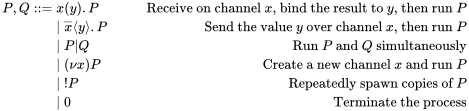
\includegraphics[width=.75\textwidth]{pi-calculus.png}    
  \end{center}
  \par\bigksip\bigskip\bigskip\bigskip\bigskip\phantom+
}
\end{frame} % pi-calc de Milner
\begin{frame}{Équivalence des paradigmes}
  Lauer et Needham on montré en 1978 que les modèles de concurrence basé sur
  procédures et les modèles basés sur messages sont équivalents (``duaux'').
  \par\bigskip
  \hfill{$\rightarrow$ \footnotesize{}cf. \textit{On the duality of operating system structures}
    H. Lauer, R. Needham 1978}
  \par\bigskip
  \begin{itemize}
  \item orienté procédures:
    \begin{itemize}
    \item beaucoup de processus, souvent créés ou détruits
    \item communication par mémoire partagée et par appels de fonction
    \item synchronisation via verrous, sémaphores ou moniteurs
    \end{itemize}
  \item orienté messages:
    \begin{itemize}
    \item peu de processus, en nombre fixe et isolés
    \item communication par messages ou événements
    \item traitement efficace des files d'attente de messages
    \end{itemize}
  \end{itemize}
\end{frame} % équivalence de Lauer-Needham

\section{Conclusion}
\minitoc
\subsection{Autres approches}
\begin{frame}
  \frametitle{Autres approches de la concurrence}
  \begin{itemize}
  % \item<1->Programmation événementielle
  % \begin{itemize}
  % \item utile pour les GUIs, mais difficile à analyser
  % \item ``event loop''
  % \item ``event handlers'' (callbacks)
  % \end{itemize}
  
  \item<1->Transactions
  \begin{itemize}
  \item idée inspirée des Bases de Donnée (langage \textbf{SQL})
  \item rendre ``atomique'' la section critique
  \item idée exploitée par exemple dans le langage \textbf{Clojure}
  \end{itemize}
  
  \item<2->Coroutines
  \begin{itemize}
  \item coroutines: des routines concurrentes pouvant ``vivre'' dans le même thread
  \item idée exploitée par exemple dans le langage \textbf{Go} (``goroutines'')
  \end{itemize}

\item<3->Modélisation de la concurrence par diagrammes
  \begin{itemize}
  \item Réseaux de Petri
  \item Diagrammes \textsc{uml} de séquence, d'activité et d'état
  \end{itemize}
  
  \end{itemize}
\end{frame}
\subsection{L'avenir de la concurrence}
\begin{frame}
  \frametitle{L'avenir de la concurrence}
  \begin{center}
    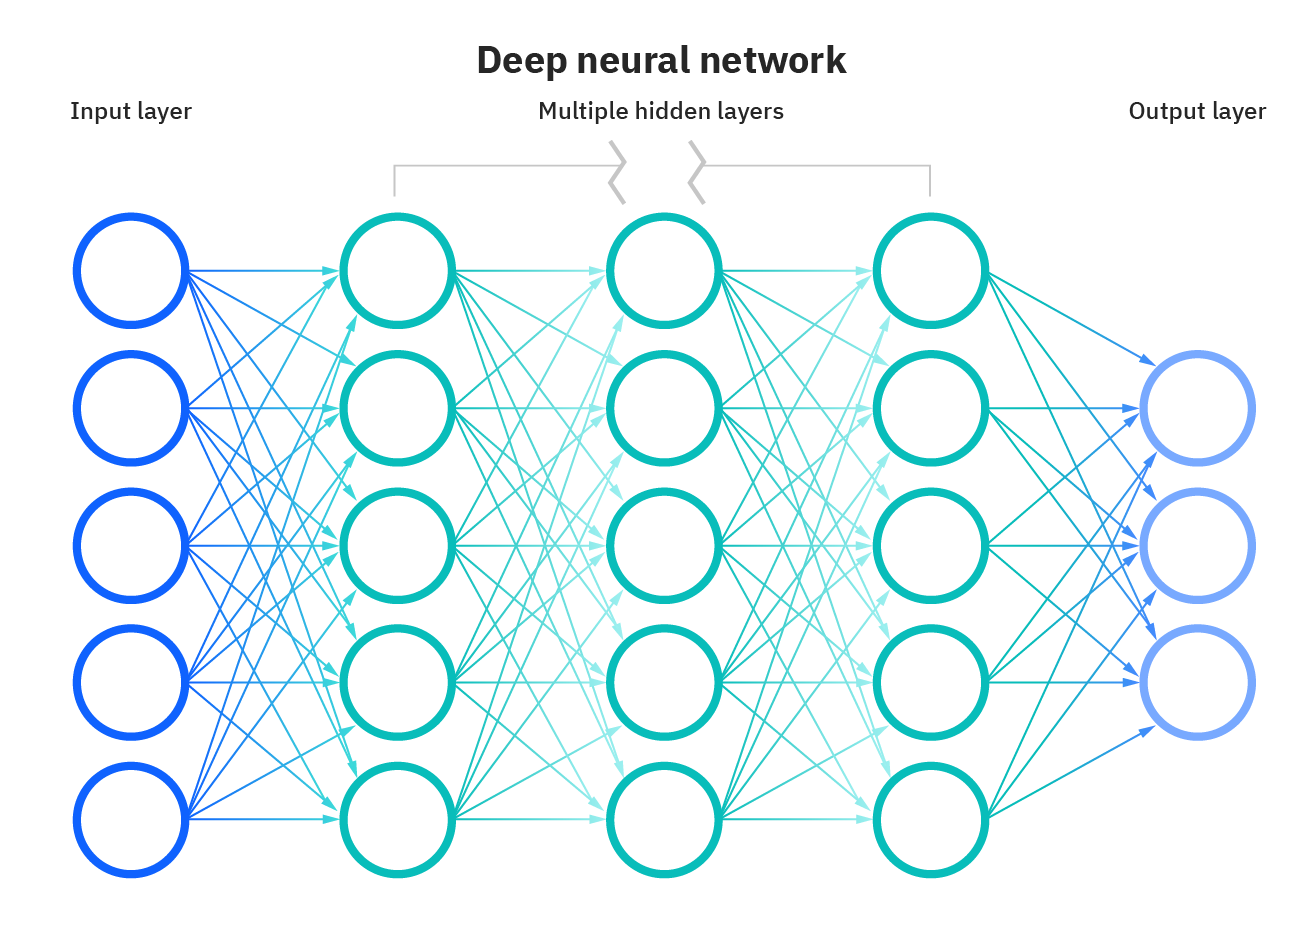
\includegraphics[width=.9\textwidth]{reseaux-neurones.png}
  \end{center}
\end{frame}


\end{document}